%	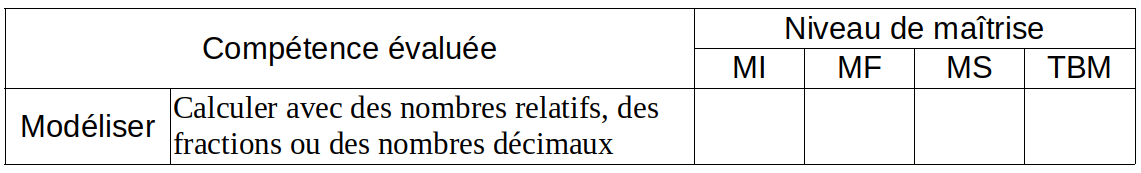
\includegraphics[scale=0.4]{competences}
	
	\section{Calculer}
	Calculer les expressions suivantes en détaillant tous les calculs:
	\begin{questions}
		
	
		\question[3]  $A = 5 + 7 \times 8 - 2$
		
		\fillwithdottedlines{6cm}
			 
		\question[3]  $B = 32 + 41 - 23 + 15$
		
		\fillwithdottedlines{6cm}
		
			\newpage
		
		%\question[4]  $C = 14 + 15 \div 3 + 25$
		
		%\fillwithdottedlines{6cm}
		
	
		
		\question[4]  $C = 49 \div 7 + 33 - 4$
		
		\fillwithdottedlines{5.5cm}
		
		\question[4]  $D = (\num{18.4} + \num{4.2} + \num{2.4}) \div 5 + \num{1.4}$
		
		\fillwithdottedlines{5.5cm}
		
	\end{questions}


	\section{Traduire}
	Traduire les expressions suivantes par une phrase, sans faire les calculs.
	\begin{questions}
	
	\question[3]  $E = 45 + 4 \times 5$
	\fillwithdottedlines{3cm}
	
	
	\question[3]  $F = (23 - 5) \times (7 + 3)$
	\fillwithdottedlines{3cm}
	
	\end{questions}